\subsection{Drift Chambers} \label{ssec:framework_dc}
Drift Chambers in general are a type of Multiwire Proportional Chambers (MPC) that use an array of wires at high voltage running through a chamber held at ground potential which is filled with gas.
Any ionized particle passing through the chamber will ionize its surrounding atoms, accelerating them across the chamber so that they can be collected by the nearest wire.
By computing the different pulses on each of these wires, the trajectory of the particle can then be estimated~\cite{sauli1977principles}.

DC differentiate themselves from MPC by the fact that they can obtain very precise measurements of the timing of the pulses from the wires along with the information commonly obtained by MPC.
This allows a more precise estimation of the distance at which the particle passed the wire and greatly improves the accuracy of the path reconstruction~\cite{blum2008particle}.

As can be seen in Figures \ref{fig:dc_horizontal_cut} and \ref{fig:dc_vertical_cut}, the CLAS12 Drift Chamber system measures the momentum of charged particles emerging from the target using a set of $18$ wire chambers distributed into $3$ regions with $6$ wire chambers each.
Each wire chamber consists of $2$ superlayers, while each superlayer of $6$ layers and each layer of $112$ wires, making up to a total of $24,192$ sense wires strung on the entire machine~\cite{mestayer2000clas}
    
    \begin{wrapfigure}{r}{0.51\textwidth}
        \centering
        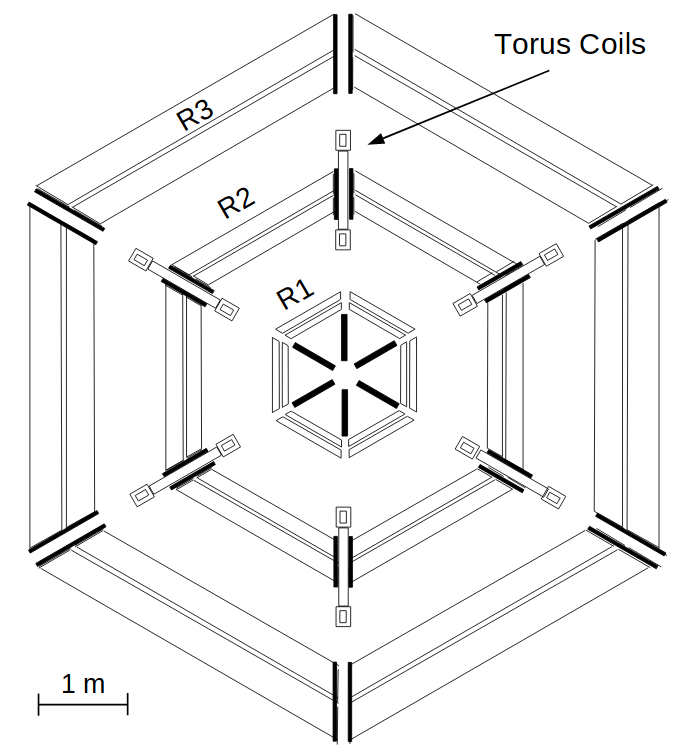
\includegraphics[width=1\textwidth]{dc/vertical_cut}
        \caption{\label{fig:dc_vertical_cut} Vertical cut through the drift chambers transverse to the beam line at the target location. Source: The CLAS Drift Chamber System~\cite{mestayer2000clas}.}
    \end{wrapfigure}

After obtaining the measurements, the DCHB and DCTB CLARA engines run to process them and deduce the tracks of the detected particles.
Pattern recognition for the DC is first done on a hit-based basis, where a hit is defined as a wire with a recorded signal.
Prior to searching for track segments (groups of hits) in each superlayer, a hit-pruning algorithm is employed to reject apparent noise, which is defined based on the number of contiguous hits in a layer.

Since the particles should go through layers close to horizontally, if many hits are detected contiguously in one layer it usually means that either the wires are malfunctioning or various wires are detecting the same particle, so unnecessary hits are rejected.

The pruned hits are then grouped into clusters, defining a cluster as a contiguous set of hits spanning through different layers in a superlayer.
A more detailed description of the cluster finding algorithm is given in Section \ref{ssec:framework_cf}.
The pairs of clusters in two adjacent superlayers are denoted as crosses.
Linear fits to these crosses serve as cluster refiners and are a preliminary step to estimating a particle's trajectory or track.

Then, a fit is done to sets of three crosses which can be linear o curved depending on the strength of the local effect of the magnetic field in the particle's trajectory.
This fit is commonly denoted as track fitting.
Track parameters are estimated in the global coordinate system of the detector from this trajectory, and are then fed as input to the Kalman Filter, which refines an estimate of the parameters of a track.

A general description of the KF algorithm is explained in Section \ref{ssec:framework_ekf}, while the specific implementation done for the track finding in CLAS12 can be read in Section \ref{ssec:framework_tf}.